% Auto-generated include snippets for CONFIRM WACV figures and tables.
% Rebuild with: PYTHONPATH=src ./.venv/bin/python paper/figures/scripts/generate_all.py

\begin{figure*}[t]
    \centering
    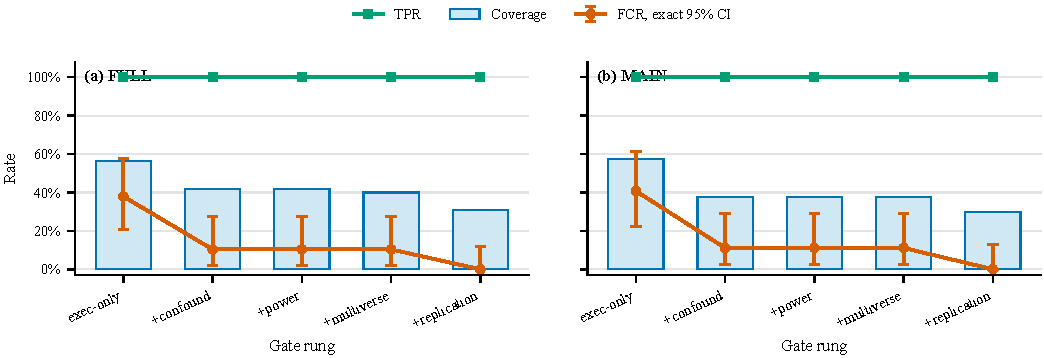
\includegraphics[width=\textwidth]{figures/fig_coverage_fcr.pdf}
    \caption{Coverage, false-confirm rate (FCR), and known-positive recall (TPR) across progressively stricter CONFIRM gate rungs for the full benchmark and main-label subset. FCR error bars are exact 95\% Clopper--Pearson intervals.}
    \label{fig:coverage_fcr}
\end{figure*}

\begin{figure*}[t]
    \centering
    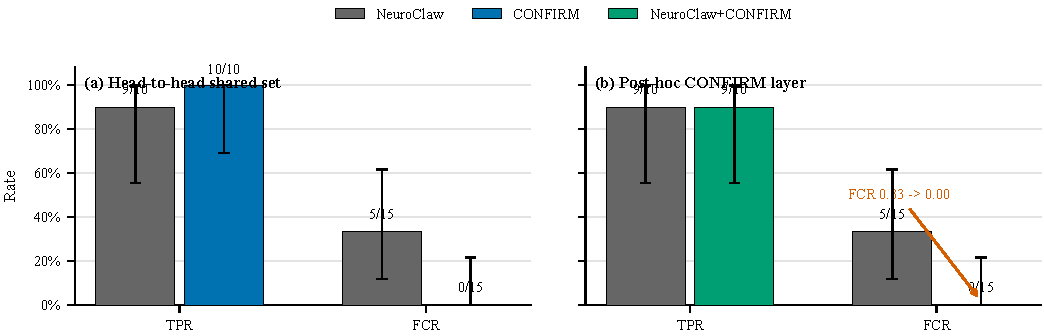
\includegraphics[width=\textwidth]{figures/fig_neuroclaw.pdf}
    \caption{Head-to-head comparison with NeuroClaw and post-hoc CONFIRM layering. Bars show TPR and FCR with exact 95\% binomial intervals; labels show count/denominator. The CONFIRM layer removes NeuroClaw false confirms while preserving the NeuroClaw positive-recall count.}
    \label{fig:neuroclaw}
\end{figure*}

\begin{figure*}[t]
    \centering
    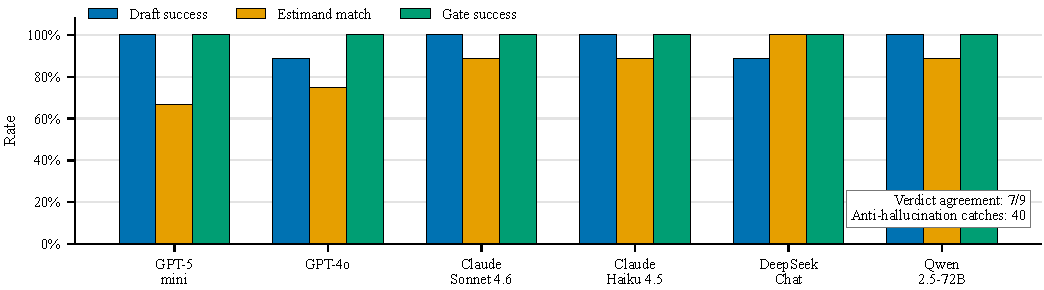
\includegraphics[width=\textwidth]{figures/fig_multillm.pdf}
    \caption{Agentic multi-LLM sweep across six models. Bars report artifact-derived draft-success, estimand-match, and gate-success rates; the inset summarizes cross-model verdict agreement and anti-hallucination catches.}
    \label{fig:multillm}
\end{figure*}

\begin{table*}[t]
\centering
\caption{Confirmed positive controls used to audit CONFIRM. Effect sizes and verdicts are read from the combined benchmark audit; standardized effects are reported when present in the artifact.}
\label{tab:positives}
\scriptsize
\setlength{\tabcolsep}{3pt}
\begin{tabular}{@{}p{0.22\textwidth}p{0.10\textwidth}p{0.14\textwidth}p{0.18\textwidth}p{0.16\textwidth}p{0.09\textwidth}p{0.07\textwidth}@{}}
\toprule
Domain & Cohorts & Outcome & Direction & Effect size & Evidence & Verdict \\
\midrule
AD hippocampal atrophy & ADNI;OASIS3 & smri\_hippocampus & negative & $\beta$=-1654.209; std=-1.716 & $p$=2.18e-112 & confirmed \\
AD entorhinal atrophy & ADNI;OASIS3 & smri\_entorhinal & negative & $\beta$=-1048.840; std=-1.582 & $p$=6.07e-89 & confirmed \\
AD middle temporal atrophy & ADNI;OASIS3 & smri\_midtemp & negative & $\beta$=-3297.989; std=-1.094 & $p$=5.73e-64 & confirmed \\
AD whole-brain atrophy & ADNI;OASIS3 & smri\_wholebrain & negative & $\beta$=-6.71e+04; std=-0.525 & $p$=1.60e-48 & confirmed \\
SZ hypoconnectivity within-network FC & COBRE;FBIRN & fc\_within\_network & negative SZ minus HC on fc\_within\_network & $\beta$=-0.074; std=-0.485 & $p$=0.001 & confirmed \\
brain aging hippocampal atrophy in CN adults & ADNI\_CN;OASIS3\_CN & smri\_hippocampus & negative & $\beta$=-65.300; std=-0.434 & $p$=4.79e-23 & confirmed \\
\bottomrule
\end{tabular}
\end{table*}


\begin{table*}[t]
\centering
\caption{Gate-ladder operating characteristics for the full benchmark and the main-label subset. Entries show rate [exact 95\% CI] with count/denominator in parentheses. TPR is known-positive recall.}
\label{tab:gate_ladder}
\scriptsize
\setlength{\tabcolsep}{4pt}
\begin{tabular}{@{}llccc@{}}
\toprule
Subset & Rung & TPR & FCR & Coverage \\
\midrule
FULL & exec-only & 1.000 [0.715, 1.000] (11/11) & 0.379 [0.207, 0.577] (11/29) & 0.564 [0.423, 0.697] (31/55) \\
 & +confound & 1.000 [0.715, 1.000] (11/11) & 0.103 [0.022, 0.274] (3/29) & 0.418 [0.287, 0.559] (23/55) \\
 & +power & 1.000 [0.715, 1.000] (11/11) & 0.103 [0.022, 0.274] (3/29) & 0.418 [0.287, 0.559] (23/55) \\
 & +multiverse & 1.000 [0.715, 1.000] (11/11) & 0.103 [0.022, 0.274] (3/29) & 0.400 [0.270, 0.541] (22/55) \\
 & +replication & 1.000 [0.715, 1.000] (11/11) & 0.000 [0.000, 0.119] (0/29) & 0.309 [0.191, 0.448] (17/55) \\
\midrule
MAIN & exec-only & 1.000 [0.692, 1.000] (10/10) & 0.407 [0.224, 0.612] (11/27) & 0.575 [0.409, 0.730] (23/40) \\
 & +confound & 1.000 [0.692, 1.000] (10/10) & 0.111 [0.024, 0.292] (3/27) & 0.375 [0.227, 0.542] (15/40) \\
 & +power & 1.000 [0.692, 1.000] (10/10) & 0.111 [0.024, 0.292] (3/27) & 0.375 [0.227, 0.542] (15/40) \\
 & +multiverse & 1.000 [0.692, 1.000] (10/10) & 0.111 [0.024, 0.292] (3/27) & 0.375 [0.227, 0.542] (15/40) \\
 & +replication & 1.000 [0.692, 1.000] (10/10) & 0.000 [0.000, 0.128] (0/27) & 0.300 [0.166, 0.465] (12/40) \\
\bottomrule
\end{tabular}
\end{table*}


\begin{table}[t]
\centering
\caption{False-confirm rate on expanded negative controls. Family rows summarize the 150 newly generated negatives; the final rows compare the prior main negatives with the combined full-gate denominator. Entries show FCR [exact 95\% CI] with count/denominator in parentheses.}
\label{tab:negatives}
\scriptsize
\setlength{\tabcolsep}{3.5pt}
\begin{tabular}{@{}p{0.43\columnwidth}cc@{}}
\toprule
Set & Count & FCR [95\% CI] \\
\midrule
random label & 0/42 & 0.000 [0.000, 0.084] \\
site confound & 0/42 & 0.000 [0.000, 0.084] \\
p fishing & 0/42 & 0.000 [0.000, 0.084] \\
underpowered & 1/21 & 0.048 [0.001, 0.238] \\
cross cohort nonreplication & 0/3 & 0.000 [0.000, 0.708] \\
\midrule
Prior main negatives & 0/27 & 0.000 [0.000, 0.128] \\
Expanded negatives & 1/150 & 0.007 [0.000, 0.037] \\
Combined main negatives & 1/177 & 0.006 [0.000, 0.031] \\
\bottomrule
\end{tabular}
\end{table}


